Walking robots offer many advantages over wheeled robots or other types
of locomotion. Wheeled or tracked vehicles are unable to access over half
of the earth's landmass \cite{BigDog}. Further, many areas in which humans
operate are designed for walking as opposed to rolling, so a successful walking
robot has increased mobility in environments designed for human walking. On the
other hand, walking robots are harder to control than their wheeled
counterparts.

Many robots have looked to biological inspiration to increase the mobility and
ease of control of robots. In particular, many biological systems have increased
redundancy to aid in balance with many animals, including dogs and cats, walking
on 4 or more legs. The inspiration taken varies from imitating gait timing to
help coordinate simple legs to completely mimicking musculoskeletal layout. The
Puppy robot (\myref{fig:Puppy}) was designed to mimic the operation of a large 
canine walking in the sagittal plane \cite{PuppyDesign}.

Another advantage that animals have over most robots is their actuators.
Biological muscles are compliant and are a key part to how animals walk. Many
robots use electric motors or hydraulic actuators to actuate joints, which can
mean that other biologically inspired design decisions aren't necessarily
optimal. Puppy chose to use pneumatic artificial muscles, which have a higher
power to weight ratio than other designs and offer similar compliance and
behavior to biological muscles \cite{Tavakoli2008}. Typically seen as a
limitation, pneumatic muscles as actuators apply force during contraction, so
they need to be used in antagonistic pairs. While designing around pneumatic muscles increases the complexity
of the robot, the muscles also allow for further bio-inspiration in the robot design
and control system.

One of the major trade offs for pneumatic muscles is that they exhibit
non-linear behavior in both static and dynamic control situations.
\cite{HuntPMuscles, DynamicPMuscles} This has
motivated the designs of new types of controllers to overcome the non-linear
behavior through adaptation in the controller. In \cite{Jahanabadi2009}, the
authors propose a system called ``Active Force Control" where a neural network
is used to learn non-linear properties of the actuator and controlled mass.
The network is run in an inner control loop and the output of the network is
used to present the control situation in a linearized fashion to an outer PID
control system. The results suggest that a system model of the nonlinear
properties of the actuators decreases positional error. The work was
applied to controlling a vertical trolley and used a neural network as a black
box for modeling the system, so there is an opportunity for improving the
system and its application to controlling Puppy's rotational joints.
In \cite{Wang2013}, a model-based controller was used to control the actuation
of a revolute joint with pneumatic muscles. The author's system allowed for
decreased antagonistic muscle overlap at high accelerations combined with a
high stiffness, high overlap controller for precise position tracking in near
static situations. This adapting system was shown to be effective in their
results; however, it does not account for estimating changing properties of the
robot system that might reduce the effectiveness of the model.

A combination of these two types of controllers offers insight into how to build
an effective joint controller for Puppy. One further area of potential
improvement over existing designs is the incorporation of biological inspiration
within the controller itself. In \cite{NickFunctionalSubnetwork}, the authors
demonstrate a method for using a dynamic, biologically accurate model of neurons
to develop models of neurons for controlling physical systems. The work in the
paper describes how to create building blocks such as arithmetic operations,
differentiation or integration. These components can then be used together to
recursively create new controller architectures that use biological inspiration
taken from literature for controlling legged robots and combine these components with an
efficient system for engineering the correct control responses. Together,
existing literature suggests that a neuron-based controller that adapts to the
properties of the muscles and the joints that it controls offers a new
architecture for more efficient and more accurate control of pneumatic muscle-
actuated robots.

\section{Task Overview}

This thesis focuses on control of joints for the canine-inspired
Puppy robot in a walking scenario. The two distinguishing physical features of 
the robot are its pneumatic muscle actuators and a design that leans heavily
on the mechanics and skeleton of canines.

\begin{figure}
\centering
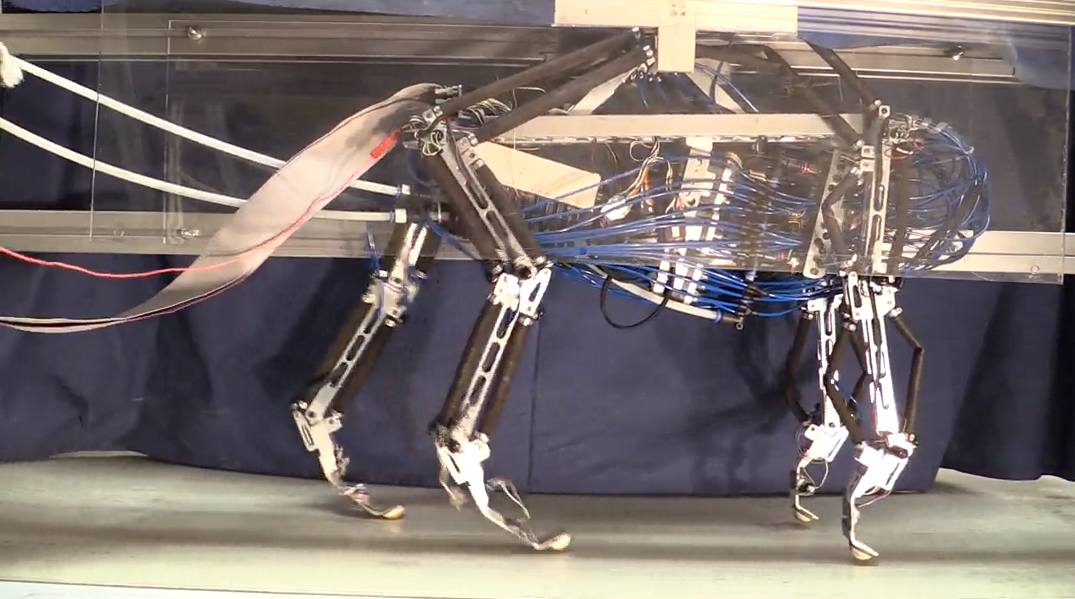
\includegraphics[width=5in]{introduction/Puppy}
\caption{The Puppy robot}
\label{fig:Puppy}
\end{figure}

\section{Specifications and Important Challenges}

There are a number of key criteria that are important for improving the behavior
of the joint controller. Based on previous work, these criteria break down as follows:

\begin{itemize}
\item Peak position during hip actuation isn't accurate (5-15 deg) 
\item Delays between sensor data off the robot -> lab view -> Animatlab -> lab
view -> robot cause tracking problems
\item Scapula drives forward motion for front legs in the reverse Z orientation
\item Improve torque profiles to eliminate external support, even close to
maximum activation
\item Better internal understanding of dynamics to match desired and intended activation
\end{itemize}

These challenges drive three key requirements for the controller.

\begin{enumerate}
\item Decrease torque errors between neuron desired model and executed torques
\item Minimize phase shift between desired and achieved trajectory
\item Decrease position error during trajectory execution to less than 5 degrees from the desired position
\end{enumerate}

These challenges and requirements define two different components and desired
behaviors for the components within the controller. First, the controller should
incorporate an internal understanding of the dynamics of the joint. This will
allow for more optimized control. This also will allow for a model-based
approach where a few key parameters can be used to summarize the behavior of the
joint so that minimal example data can be used to finely tune the parameters and
model. Without an internal understanding of the dynamics, the controller would have to
use an arbitrarily complex neuron system to model an arbitrary behavior that may
over fit to the idiosyncrasies of a few data points and not generalize
effectively to continued modeling of the joint.

Second, the controller should perform internal optimization to provide an
improved output. There are multiple ways that this optimization can occur, but
an internal optimization step built into the controller will allow for the joint
to adapt and be more efficient across multiple behaviors where a simple
controller, such as a proportional controller, is statically tuned for a single
situation and will either be inefficient or inaccurate as the environment
changes. Each step on a walking robot is potentially different, so a static
controller will almost certainly be continually sub-optimal.

Additionally, an internally optimizing controller with a model of joint dynamics can
optimize for the estimated position of a joint at a time ahead of the current
sensor data. This means that, on a system with a known delay for sensor data
leaving the robot and control commands arriving at the robot, the controller can
control the robot as if it were already at the time in the future where the
joint will be instead of at the point in the past where the joint was when the
sensor data was read.

\section{This Work}

This work continues with a review of surrounding and supporting literature in
\myref{chap:lit_review}.

\myref{chap:controller_design} 
discusses the design of a new type 
of controller that incorporates the
design goals of understanding the dynamics, projecting forward in time and
optimizing the controlled output based on the understanding of dynamics.

\myref{chap:neuron_design} discusses the implementation of the controller within 
a synthetic nervous system
simulation. This discussion talks about some simplifications and approximations
that were made in the process, as well as areas of the network that are more
complex improvements over the controller design discussed in \Cref{chap:controller_design}.

\myref{chap:methods} discusses the methods used to design, iterate, test and
validate the controller designs.

\myref{chap:results} discusses the results of testing the controllers.

\myref{chap:conclusion} discusses the conclusions and future work.
